\section{Background} \label{sec:background}

This section first presents the background of \smr, and then introduces \dmt 
with the actual \parrot runtime \xxx leverages.

\subsection{State Machine Replication} \label{sec:smr}

\emph{State machine replication (\smr)} is a powerful fault-tolerance
concept.  It models a program as a deterministic state machine, where
states are important program data and the transitions are deterministic
executions of program code under input requests.  \smr runs replicas of
this state machine on multiple nodes, tolerating many possible node and
network failures.  To keep the replicas consistent, it invokes a
distributed consensus protocol (typically \paxos~\cite{paxos}) to ensure
that a quorum (typically majority) of the replicas agree on the input
request sequence; under the deterministic execution assumption, this
quorum of replicas must reach the same exact state.  \smr is proven safe
in theory, and provides high availability in practice.

\subsection{Deterministic Multithreading} \label{sec:dmt}

\dmt~\cite{dpj:oopsla09, 
dmp:asplos09, kendo:asplos09, coredet:asplos10, dos:osdi10, ddos:asplos13, 
ics:oopsla13} is an advanced threading technique that enforces the same 
schedule 
on the same inputs.  This technique typically maintains a \emph{logical
  time}\footnote{Though related, the logical time in \dmt is not to be
  confused with the logical time in distributed
  systems~\cite{lamportclock}.} that advances deterministically based on
the code run.  It allows a thread to synchronize only at deterministic
logical times.  By induction, it makes an entire multithreaded execution
deterministic.  The overhead of \dmt is typically moderate: one recent
\dmt system, \parrot~\cite{parrot:sosp13}, incurs an average of 12.7\%
overhead on a wide range of 108 popular multithreaded programs on 24-core
machines.

\section{\xxx Overview} \label{sec:overview}

This section first introduces \xxx's architecture with its key components, and 
then discusses which types of anlyses are suitable to run in \xxx. We mainly 
consider server applications (\eg, \apache and \clamav) because they provide 
online service and thus require significant analyses to guarantee software 
quality. Utility programs can also be easily run in our \xxx.

\subsection{Architecture} \label{sec:arch}

\xxx's deployment is similar to a typical \smr's. In a \xxx-replicated
system, a set of 2\v{f}+1 machines (nodes) are set up within a LAN,
and each node runs an instance of \xxx containing the same server
program running with or without an anlysis tool. Once the \xxx system starts, 
one node becomes the \emph{primary} node which proposes the order of requests 
to execute, and the others become backup nodes which follow the primary's 
proposals. Up to \v{f} nodes run an heavyweight anlysis tool on each, so at 
least \v{f}+1 nodes run the native application or lightweight analyses so that 
they can reach consensus on inputs and process requests fast. An arbitrary 
number of clients in LAN or WAN send network requests to the primary and get 
responses. 


\begin{figure}[t]
\vspace{.20in}
\centering
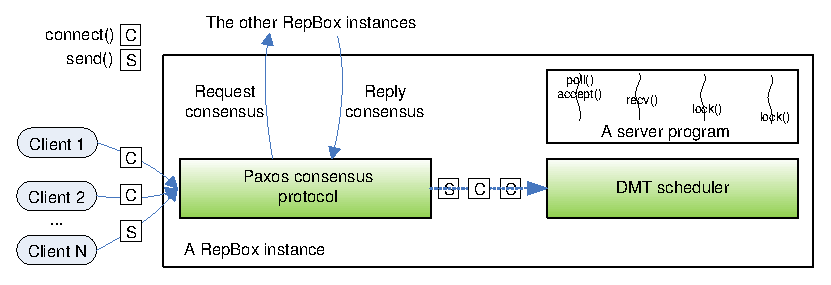
\includegraphics[width=.5\textwidth]{figures/arch}
\vspace{-.20in}
\caption{{\em The \xxx Architecture.} \xxx components are shaded (and in
  green).} \label{fig:arch}
\vspace{-.05in}
\end{figure}

Figure~\ref{fig:arch} shows an instance of \xxx running on 
each node. The abstraction contains three main components, the \paxos consensus 
component, the \dmt scheduler, the checkpointer component. A server program 
runs transparently in a \xxx instance with or without an analysis. Neither the 
server or the analysis is aware of of \xxx's components.

To support general server programs, \xxx chooses the POSIX socket API as
consensus interface. \xxx enforces two kinds of orders for socket
operations.  For requests coming from the clients, such as \connect and
\send requests, \xxx enforces that all nodes see the same totally ordered
sequence of these requests using the \paxos and socket API interposition
components.  (\xxx does not need to order the blocking socket operations
in the clients because we mainly focus on analyses for server applications.)


The \paxos consensus component is a \xxx instance's gateway.  It accepts socket
requests from the clients and invoke a \paxos consensus instance on this 
operation. Once a consensus is reached. This component is also the only \xxx 
component that communicates among different \xxx instances. For practicality, 
\xxx uses a well-known \paxos engineering approach~\cite{paxos:practical} in 
which only the primary invokes consensus request during normal operations.

The \dmt component runs within the same process as a server replica, and
enforces the same logical clocks for inter-thread communication
operations. \xxx leverages the \parrot~\cite{parrot:sosp13} \dmt runtime
system because it was shown to run fast on a wide range of 108 popular
multithreaded programs. We choose this \dmt runtime because it is fast (\ie, 
12.7\% overhead for a wide range of 108 popular multithreaded programs) and 
transparent to the application.

Specifically, \parrot uses a runtime technique called \ldpreload to dynamically 
intercept \pthread synchronizations (\eg, \mutexlock) issued by an executable 
and enforces a well-define, round-robin schedule on these synchronization 
operations for all threads, practically eliminating nondeterminism in thread
synchronizations. Although \parrot is not designed to resolve data races
deterministically, \xxx's replication tolerates data races that have
fail-stop consequences.  \xxx augments the \dmt component to schedule the
return points of socket operations in server replicas, too, to ensure that
requests are admitted exactly at the same logical time across replicas.

The checkpointer component is invoked every minute in a non-primary node that 
is running the native application and nodes that are running an analysis. Each 
checkpoint is associated with the index of the last executed socket operation, 
so that \xxx can consistently match up with the execution states of native 
executions and various analysis executions. To perform checkpoints 
transparently without affecting application's executions and analyses, \xxx 
leverages \criu, a popular, open source process checkpoint tool that supports 
CPU registers, memory, etc. Each checkpoint operation is only performed on the 
server program and the \dmt schculer; the \paxos consensus component does not 
require checkpoints because we explicitly design it to be stateless (all socket 
operations have been persisitently logged).

% Our model. Multiple writer multiple reader.

\subsection{Discussion} \label{sec:discuss}

\subsubsection{What Types of Analyses are Suitable to Run in \xxx?} 
\label{sec:analysis-types}

We envision that an analysis is suitable for \xxx if: (1) it can be done 
loosely coupled with the actual execution, and (2) it does not schedule 
conflicting order of \pthread synchronizations that \xxx's \dmt runtime 
enforces. Many reliability analyses, including data race detection, profiling, 
and logging meet this requirement. Some security analysis such as control flow 
integrity is not suitable for \xxx because it monitors the execution 
synchronously for each control flow transfer. In addition, some security 
analysis such as information leakage protection are not 
suitable for \xxx because the actual execution may probably run faster than the 
analysis and leak information to clients before the analysis detects the 
leakage. Nevertheless, many security tools such as use-after-free 
vulnerabilities can be deployed in \xxx.

\subsubsection{Can \xxx Strengthen Existing Analyses?} 
\label{sec:strengthen-analysis}

\xxx is not only transparent to analysis tools, but has the potential to 
improve the strengths of existing analyses by its performance benefit. 
Previously, to mitigate the huge performance slowdown, some analysis tool 
developers sometimes have to sacrifice some strenghths of the analysis. For 
instance, ThreadSanitizer\cite{tsan}, one of the most practical race detectors, 
only records the last few accesses as the access history for each memory byte 
instead of the full access history, because analyzing the full access history 
is extremely heavyweight (\eg, 200X slowdown for some programs they evaluated). 
However, ignoring part of the access history may miss data races. With \xxx, 
developers can now analyze the full memory access history.

\smr provides an extra significant fault-tolerance benefit for \xxx. Existing 
reliability and security analyses tend to expose or detect harmful defeats in 
an application, which may crash the application. In addition, the actual 
executions across different nodes may fail as well due to hardware or OS 
failures. With \xxx's \smr architecture, the sequence of inputs are 
persistently and consistently enforced across replicas, and failing minor 
nodes (either an analysis or an actual execution node) do not affec the other 
nodes' executions and anlyses.

\subsubsection{Can Existing Analyses Strengthen \xxx?} 
\label{sec:strengthen-crane}

Interestingly, analyses running in \xxx can benefit \xxx's \dmt runtime and 
improves its performance. Specifically, a \dmt runtime enforcing the order of 
shared memory accesses is fully deterministic even with data races, but it 
incurs prohibitive slowdown (\eg, 5X to 124X slowdown evaluated 
in~\cite{parrot:sosp13}) because typical applications have intensive amounts of 
shared memory accesses. A \dmt runtime enforcing the order for synchronizations 
only can run efficiently (\eg, less than 16\% overhead in~\cite{kendo:asplos09, 
tern:osdi10, parrot:sosp13}) because synchronizations are rare and the 
remaining of the code can still run in parallel, but this \dmt is only 
deterministic when no races occur. Despite much effort~\cite{dthreads:sosp11, 
peregrine:sosp11, determinator:osdi10}, there is still no a simple and 
deployable approach to enforce fully Deterministic and efficient \dmt schddules.

Fortunately, \xxx's replication architecture can address this problem with a 
simple and thorough approach by deploying a race detector in one replica, then 
the \dmt no longers need to schedule shared memory accesses. If the race 
detector reports a race, developers can easily diagnose and fix it because 
synchronization schedules enforced by \dmt already make the race easily 
reproducable~\cite{pres:sosp09}. By enforcing the same synchronization 
schedules across replicas, the race detection results consistently hold for all 
replicas. In sum, \xxx and race detection tools can form a mutual-beneficial 
eco-system.
